\chapter{Multi-Viewpoint Solar Radio Observations: Integrating Space-based and Ground-based Data for Coronal Diagnostics}
\label{chapter1}
%\maketitle{Integrating LOFAR and PSP Observations for Coronal Diagnostics}

\section{Introduction}
Type III radio bursts are manifestations of transient energetic electron beams injected into the solar corona, propagating along the interplanetary magnetic field (IMF) lines \citep{ergun98, pick6, reid20}. As these beams traverse the corona, they trigger plasma waves (also known as Langmuir waves) that are then transformed into radio emission at the local plasma frequency or its harmonic components \citep{melrose17}. 
In the radio spectrograms, type III bursts are usually observed as intense emissions that drift in frequency over timescales of several seconds to minutes and over a wide range of frequencies, from metric to decametric wavelengths \citep{wild50, lecacheux89, bonnin8}, making them detectable by ground-based instruments on Earth and various spacecraft within the heliosphere. 
The frequency of the radio emission is directly related to the plasma density, making type III bursts a valuable diagnostic tool for examining the inner heliosphere and the processes that drive solar active phenomena, such as solar flares and coronal mass ejections \citep{reid14, kontar17}.

The electron beams follow open magnetic field lines and can persist well beyond 1 astronomical unit (AU) (e.g., \citet{dulk85, boudjada20}), offering in situ insights into the burst and ambient conditions of the heliosphere, including electron density, radio frequency drift, speed of the electron beams and even potential direct detection of Langmuir waves (see \citet{gurnett76, gurnett77} and \citet{reid14} and references within). In addition, tracing the path of type III bursts provides a map of the density structure of the heliosphere, serving as a foundation for developing and testing density models.
Since radio observations below $\sim$10 MHz cannot be accomplished from the ground, it is important to combine high- and low-frequency observations from ground-based and space-borne instruments.
In this work, we perform a study of several type III radio bursts that occurred in close succession on April 3, 2019. We use remote observations of type III radio bursts detected by the Low-Frequency Array \citep[LOFAR]{lofar13} ground-based radio telescope and the Parker Solar Probe \citep[PSP]{fox16} spacecraft during Encounter 2 to study the sources of these radio emissions and to investigate the physical conditions responsible for their generation. Additionally, we incorporate results of two steady-state models of the solar corona: the potential field source surface (PFSS) model \citep{altschuler1969magnetic, schatten1969model} and the magnetohydrodynamic algorithm outside a sphere (MAS) model \citep{mhd99}, to gain a better understanding of the coronal magnetic environment and its role in the acceleration of electrons. 
The ground-based LOFAR imaging observations provide valuable insight into the actual location of the burst sources. This research aims to expand upon current knowledge of the electron beams responsible for triggering type III radio bursts and the coronal conditions they experience. Gaining a deeper insight into this aspect is vital in comprehending other solar phenomena, such as solar energetic particles and solar wind, and how they influence the near-Earth space environment.

A number of recent studies investigate the physical mechanisms responsible for the generation of solar type III radio bursts. 
For example, \citet{chen13} investigated the association of type III bursts with flaring activities in February 2011, via combined multi-wavelength observation from the Solar Dynamic Observatory (SDO) instruments, as well as Wind/WAVE and ground-based instruments. They found that the SDO measurements indicated that type III emission was correlated with a hot plasma (7 MK) at the extreme ultraviolet (EUV) jet's footpoint. 
By using a triangulation method with the Wind and the twin STEREO spacecraft, \citet{bonnin8} reported the first measurements of the beaming characteristics for two type III bursts between 2007-2008, assuming the source was located near the ecliptic plane (see also \citet{reiner9}). They concluded that the individual type III bursts have a broad beaming pattern that is roughly parallel to the Parker spiral magnetic field line at the source.
\citet{saint12} conducted a study on almost 10,000 type III bursts observed by the Nancay Radioheliograph between 1998 and 2008. Their analysis revealed discrepancies in the location of type III sources that may have been caused by a tilted magnetic field. Additionally, they found that the average energy released during type III bursts throughout a solar cycle could be comparable to the energy produced by non-thermal bremsstrahlung mechanisms in nano-flares.
\citet{morosan17} utilized LOFAR data to investigate the statistical characteristics of over 800 type III radio bursts within an eight-hour period on July 9, 2013. They discovered that the drift rates of type III bursts were twice that of type S bursts and plasma emission was the primary emission mechanism for both types.

\citet{pulupa20} introduced a statistical overview of type III radio bursts during the first two PSP solar encounters. While the first encounter in November 2018 revealed a small number of bursts, the second encounter in April 2019 exhibited frequent type III bursts, including continuous occurrences during noise storms. They reported the characteristics of type III bursts with spectral and polarization analysis.

\citet{Krupar_2020} performed a statistical survey of 30 type III radio bursts detected by PSP during the second encounter in April 2019 and estimated their decay times, which were used to estimate the relative electron density fluctuations in the solar wind. They localized radio sources using a polarization-based-radio triangulation technique, which placed the sources near the modeled Parker spiral rooted in the active region AR12738 behind the plane of the sky as seen from Earth.

\citet{Cattell_2021} explored correlations between type III radio bursts and EUV emission in the solar corona. Using coordinated observations from PSP, SDO, and Nuclear Spectroscopic Telescope Array (NuSTAR) on April 12, 2019, they identified periodicities in EUV emission correlated with type III burst rates. The findings suggested impulsive events causing heating and cooling in the corona, possibly nano-flares, despite the absence of observable flares in X-ray and EUV data, which implies periodic non-thermal electron acceleration processes associated with small-scale impulsive events.

\citet{harra2021active} explored the origin of the type III radio bursts we are tackling in this paper and found that electron beams that triggered radio bursts may have emanated from the periphery of an active region that showed significant blue-shifted plasma.
More recently, \citet{badman22} observed a distinct type III radio burst using the PSP and LOFAR between 0.1 and 80 MHz on April 9, 2019, around 12:40 UT, six days after the occurrence of the event analyzed in our study. While no detectable flare activity was linked with the event, a type III noise storm was ongoing during the PSP encounter 2. The authors determined the type III trajectory and reconstructed its source using observations from Wind and STEREO spacecraft, as well as measuring related electron enhancement in situ.

In the last few years, we have witnessed the emergence of modern instruments, such as LOFAR and PSP, that have allowed for the observation of solar radio emissions with higher sensitivity from a better vantage point. Although type III bursts have been extensively studied \citep{dabrowski21}, there are still some unresolved issues regarding the exact mechanism of type III emissions.
For example, it is not yet clear how the electrons are accelerated to the high energies required to generate type III radio bursts or what role the coronal magnetic field plays in this process.
Furthermore, there are inconsistencies between the observations and the models, which need to be resolved in order to gain a more complete understanding of the dynamics of the solar corona. Examples of these inconsistencies are the origin of the type III radio bursts and the discrepancy between the estimated plasma densities from the models and the observations. This paper aims to address these unresolved challenges by using new observations from LOFAR and PSP and models of the solar corona to study the physical mechanisms responsible for the generation of type III bursts.
The data analysis includes a combination of radio spectroscopy and imaging techniques to study the frequency, temporal and spatial variations of the radio bursts. 

The paper is organized as follows. In Section~\ref{s_obs}, we describe the observations of type III radio bursts made with LOFAR and PSP. In Section~\ref{s_methods} we explain the data analysis and modeling techniques used to study these events. In Section~\ref{s_results}, we present the results of our analysis, including an investigation of the potential physical mechanisms responsible for the generation of type III radio bursts and a comparison of the observations with models of the solar corona. Finally, in Section~\ref{s_conclusions}, we summarize our findings and discuss their implications.

\section{Observations}
\label{s_obs}
A number of studies focused on observing the solar radio emissions during the second encounter of the PSP in late 2019 \citep{Krupar_2020, pulupa20, Cattell_2021, harra2021active, badman22}. In this study, our primary emphasis is directed towards investigating a set of type III radio bursts that took place on April 3, 2019, during the time interval spanning from $\sim$12:10 to 12:50 UT. This period coincided with the presence of two distinct active regions (ARs) on the Sun, denoted as AR12737 and AR12738. 
AR12737 was situated on the Sun's near side at coordinates E12$^o$N06$^o$. Notably, this region had eight sunspots and exhibited a $\beta$ magnetic configuration according to the Hale magnetic classification \citep{hale_1919}. On the other hand, AR12738 was positioned on the solar far side at coordinates E140$^o$N02$^o$. Due to its remote location, detailed observations of the magnetic configuration and activity within AR12738 were unattainable in this time frame.

We observed a group of intense type III radio bursts by four instruments (Wind/WAVES, PSP/FIELDS, STEREO-A/SWAVES, and LOFAR/LBA) via a regular survey. In Figure~\ref{fig_alldyspec}, we show the first type III burst within the time of this study as observed by the four instruments. By taking the second derivative of the light curve at a specific frequency channels, we determined the start time of the burst, which is denoted by the vertical red dashed line. The frequency bands used for obtaining the start time at each instrument are as follows: 6.97 MHz (Wind), 7.03 MHz (STEREO), 5.03 MHz (PSP), and 40.16 MHz (LOFAR).

We checked the relative orientations of the instruments with respect to Earth (Fig.~\ref{locations}). Since the PSP and STEREO spacecraft were almost aligned (close in an angular sense) with the Sun, the STEREO/EUVI image could be taken as what PSP would see (Fig.~\ref{soldisk_xrs}).
Figure~\ref{soldisk_xrs} shows how the solar disk looks like from the Earth perspective (using the SDO/AIA instrument) and from the eastern side where the PSP and STEREO were located at that time (using the STEREO/EUVI instrument).
The right panel shows a closer view of AR12737 with the contours of the photospheric magnetic field obtained from the Helioseismic and Magnetic Imager (HMI) on board SDO.
From the GOES-15/XRS and SDO/EVE instruments in the panels below, they also confirm that there is no flaring activity at that time.

The solar disk was quiet, including only one AR that is visible with no X-rays and no EUV transient emissions over this period.
Nevertheless, the very sensitive LOFAR telescope detected a number of bursts close to noon. We checked PSP data, and we found bursts there as well.
Meanwhile, from the EUVI and AIA images, we see that there are numerous small localized regions of relatively higher intensity (i.e., likely small-scale coronal brightenings spots or campfires; see \citet{young18, madjarska19, berghmans21}).
In the next subsections, we introduce the PSP and LOFAR instruments and their observations of the radio bursts.
\begin{figure}
\centering
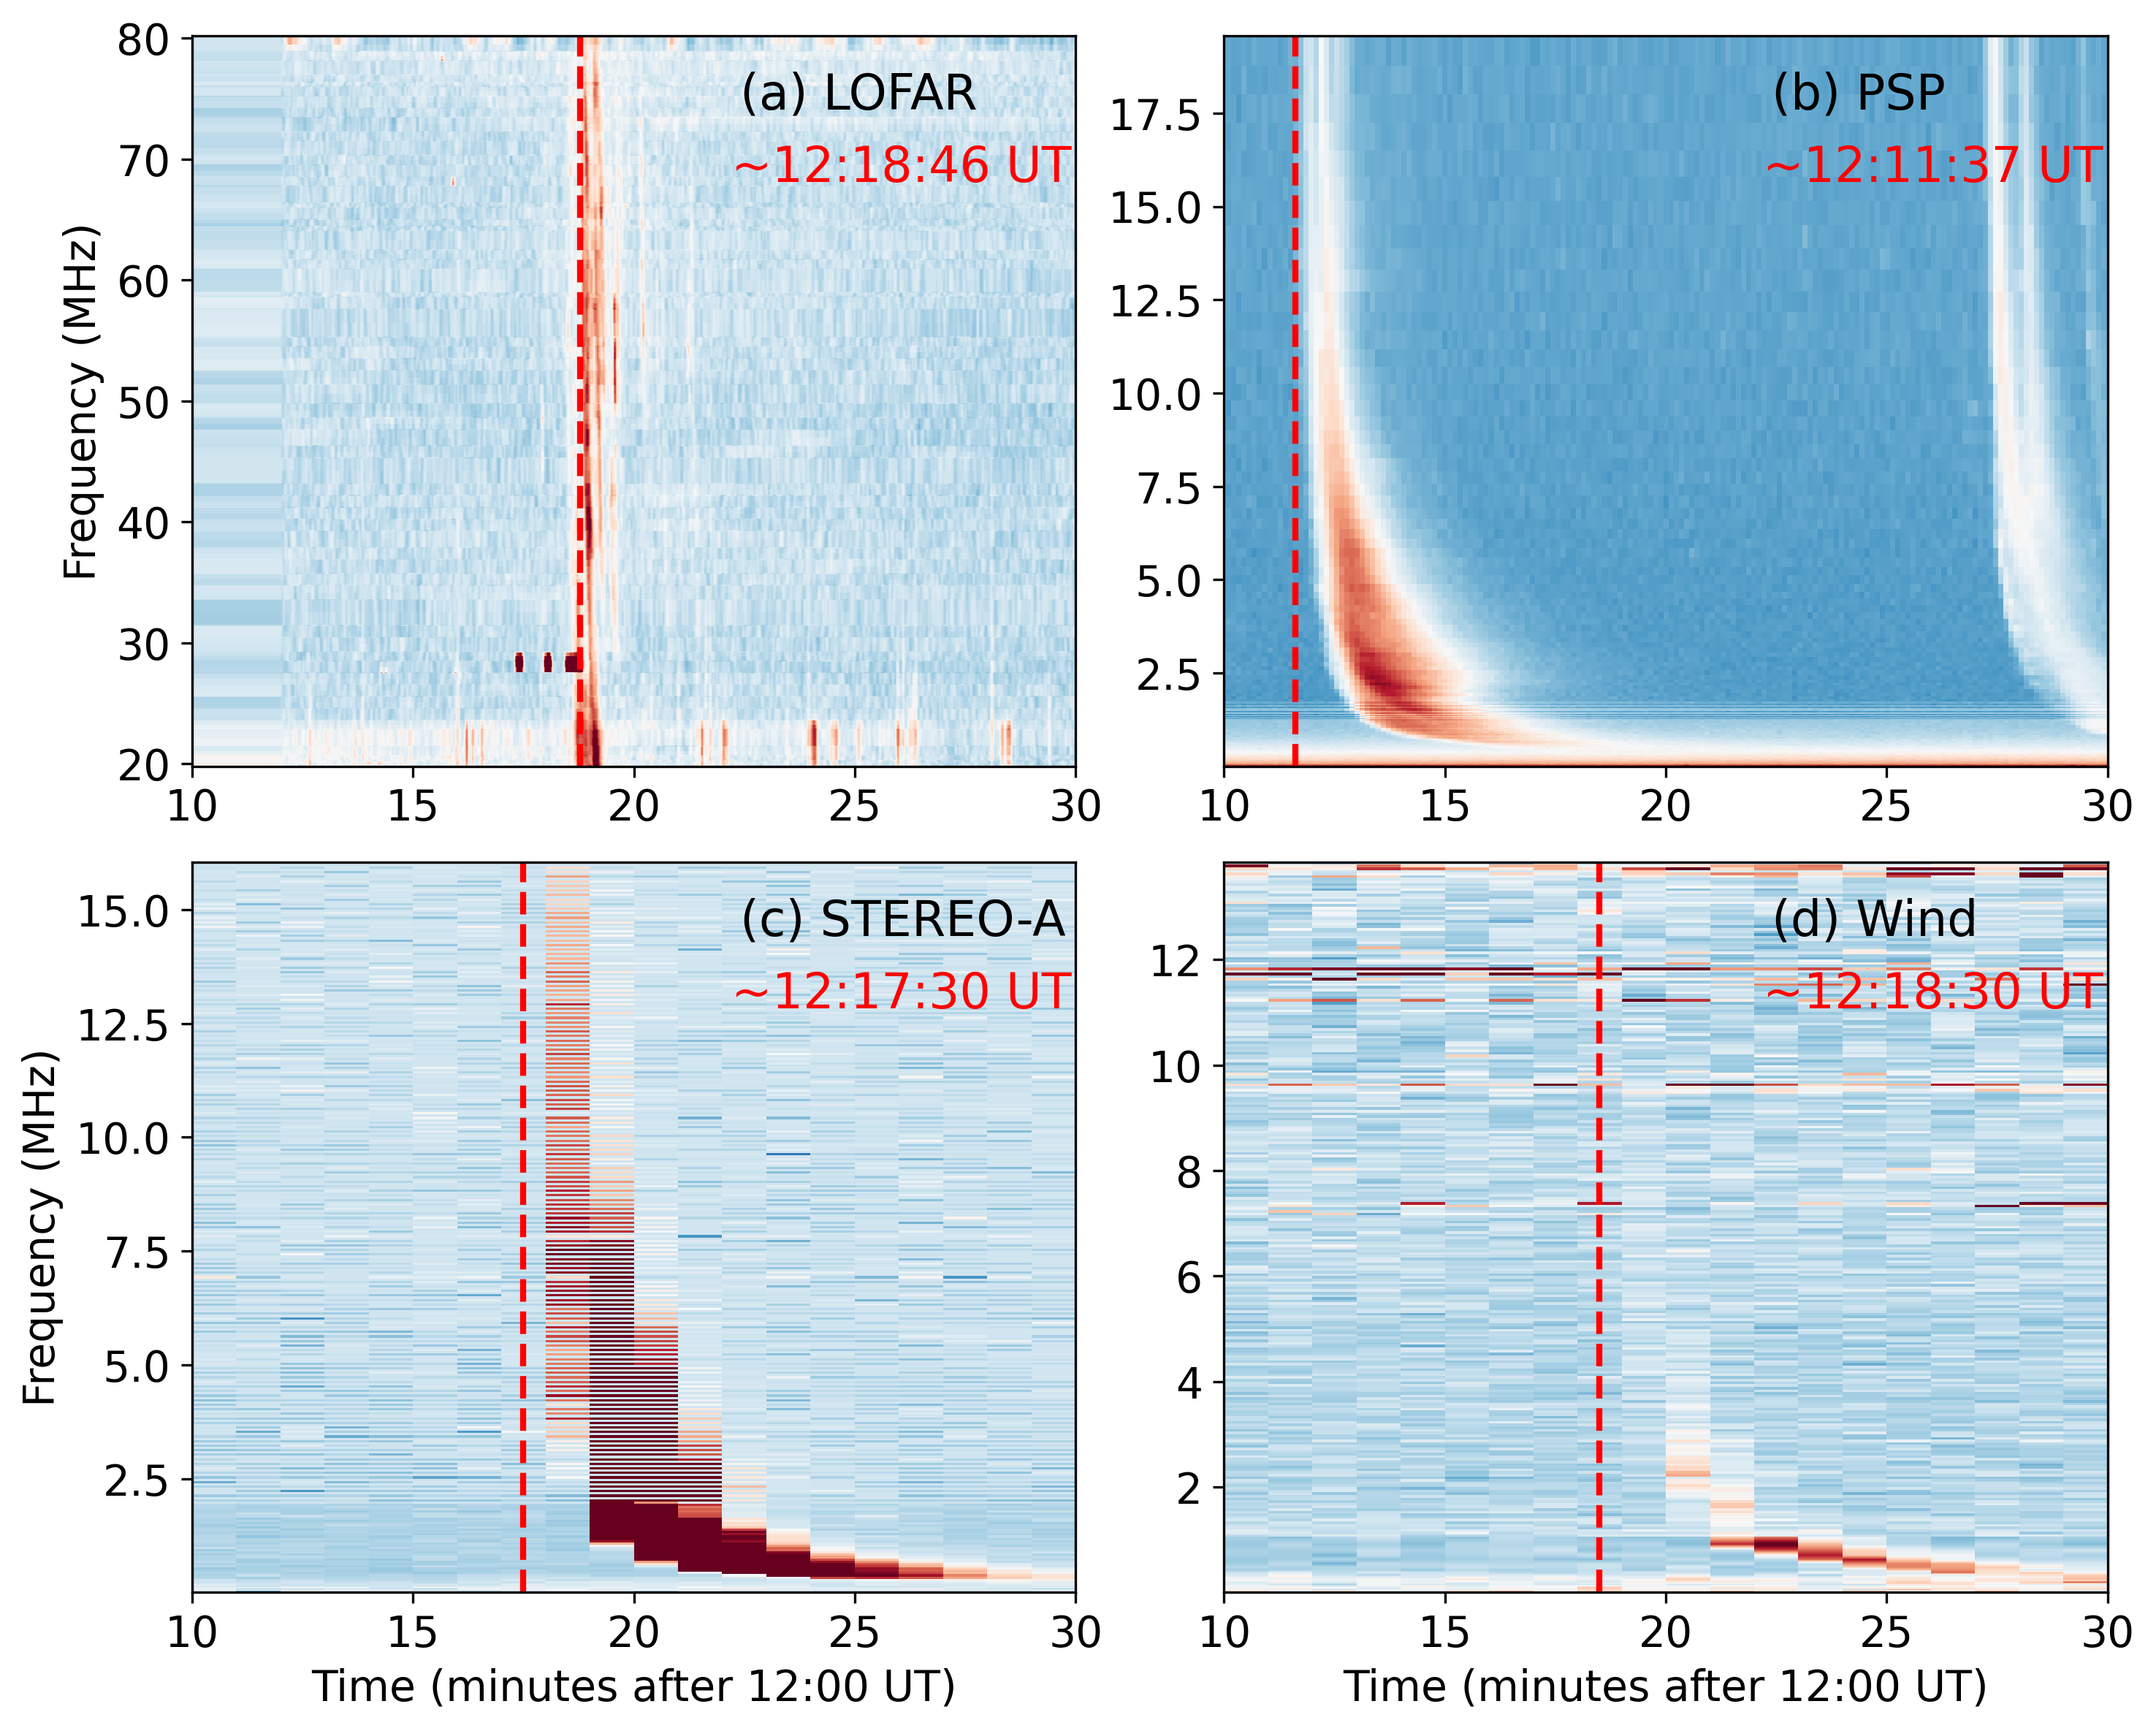
\includegraphics[width=0.9\hsize]{figs/ch2/all_dyspec.png}
\caption{Radio dynamic spectra for a single burst obtained from multiple instruments. The top-left panel is from the LOFAR/LBA instrument, the top-right is from the PSP/FIELDS instrument, the bottom-left is from the STEREO/SWAVES instrument, and the bottom-right is from the Wind/WAVES. The vertical red dashed line denotes the start time of the burst.}
\label{fig_alldyspec}
\end{figure}

\begin{figure}
\centering
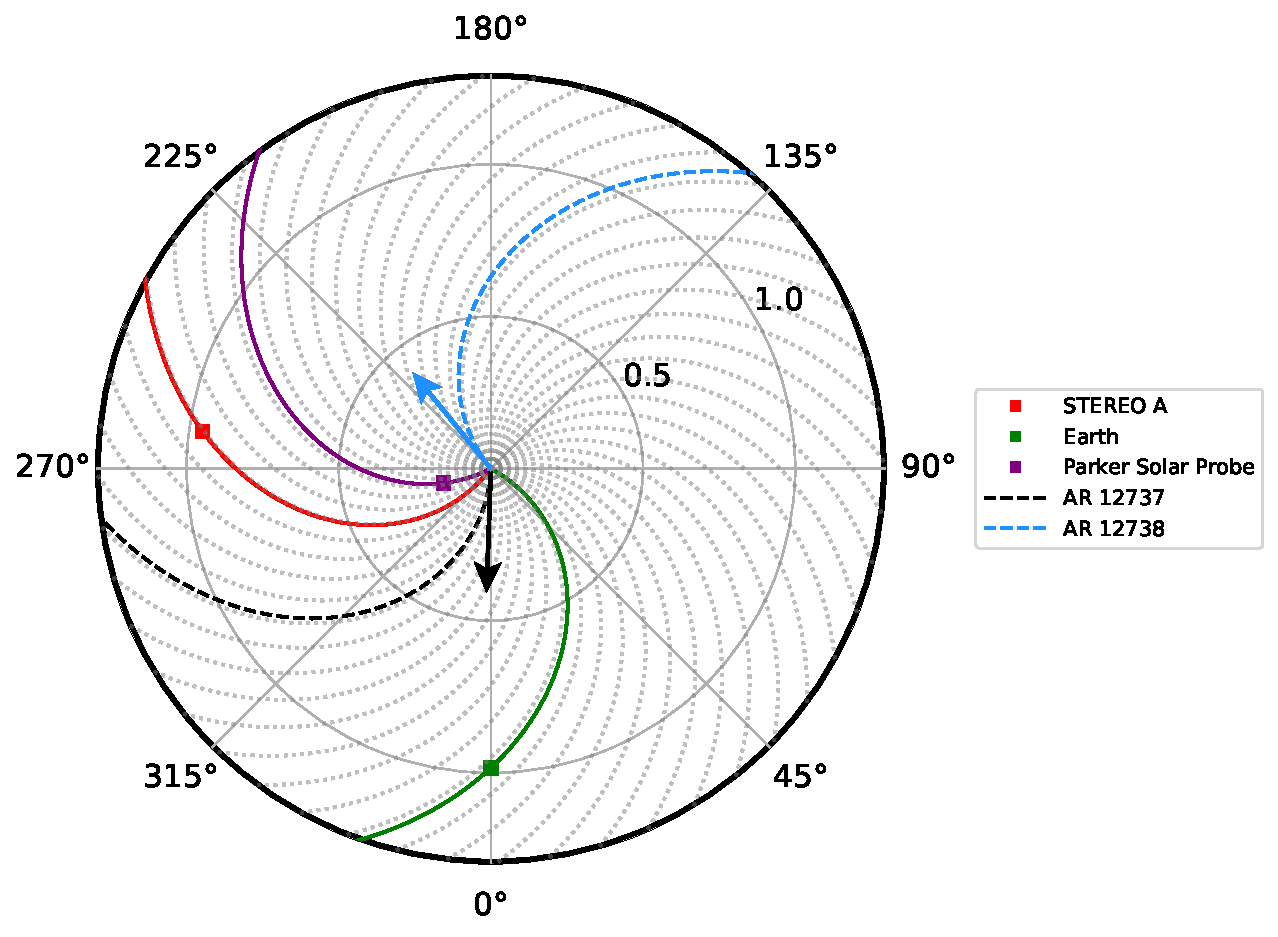
\includegraphics[width=0.8\hsize]{figs/ch2/solarMach.pdf}
  \caption{Top view of the spacecraft positions in the ecliptic plane at 12:15 UT on April 3, 2019, with the Sun-Earth line as the reference point for longitude. The Earth's location is representative of the positions of LOFAR, Wind/WAVES, and GOES-15/XRS instruments. The spacecraft were connected back to the Sun by a 400 km/s reference Parker Spiral. The black arrow represents the longitude of AR12737 and the blue arrow represents the longitude of the AR12738. The gray dotted lines are the background Parker spiral field lines. The black dashed spiral shows the field line connected to the AR12737, and the blue dashed spiral is connected to the AR12738. The figure is generated using the Solar MAgnetic Connection Haus (\href{https://github.com/jgieseler/solarmach}{Solar-MACH}) tool \citep{Gieseler2023}.}
     \label{locations}
\end{figure}

\begin{figure*}[ht]
\centering
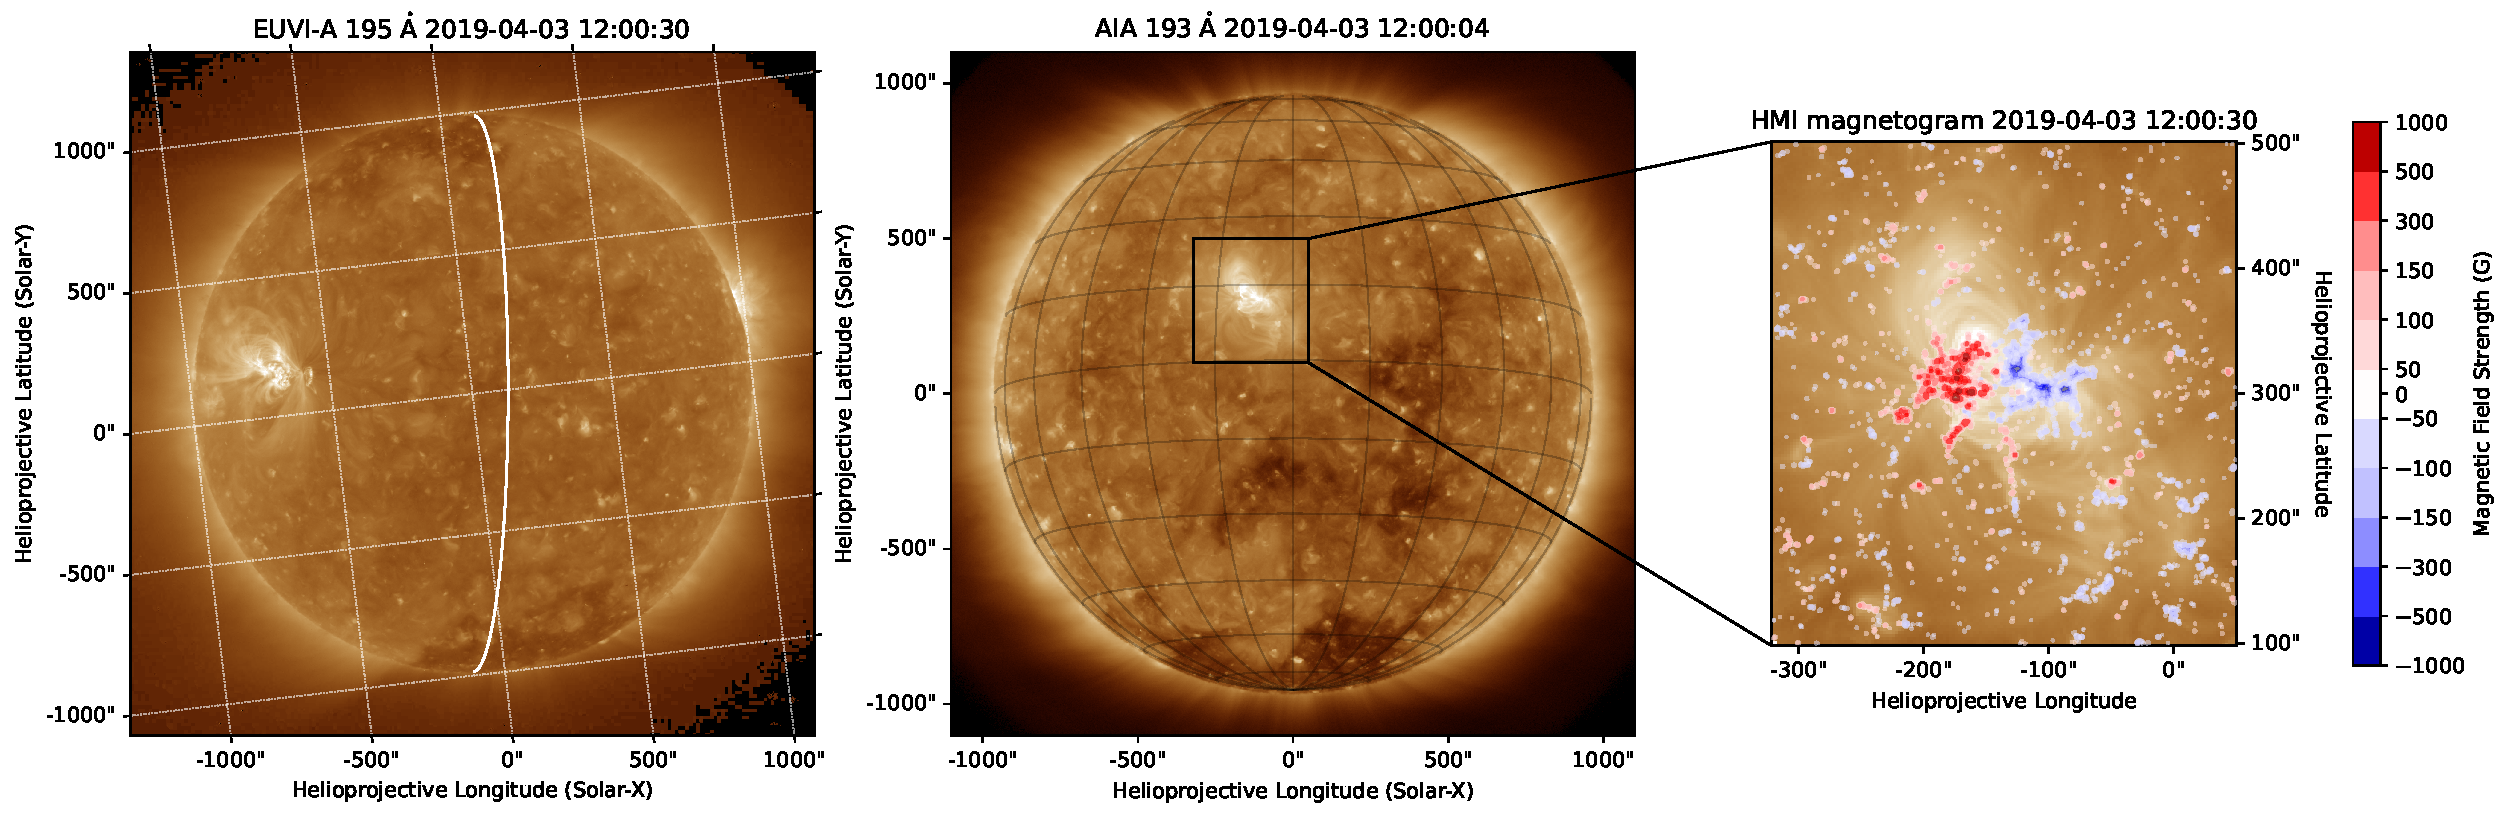
\includegraphics[width=\hsize]{figs/ch2/aia_sta_cutout.pdf}
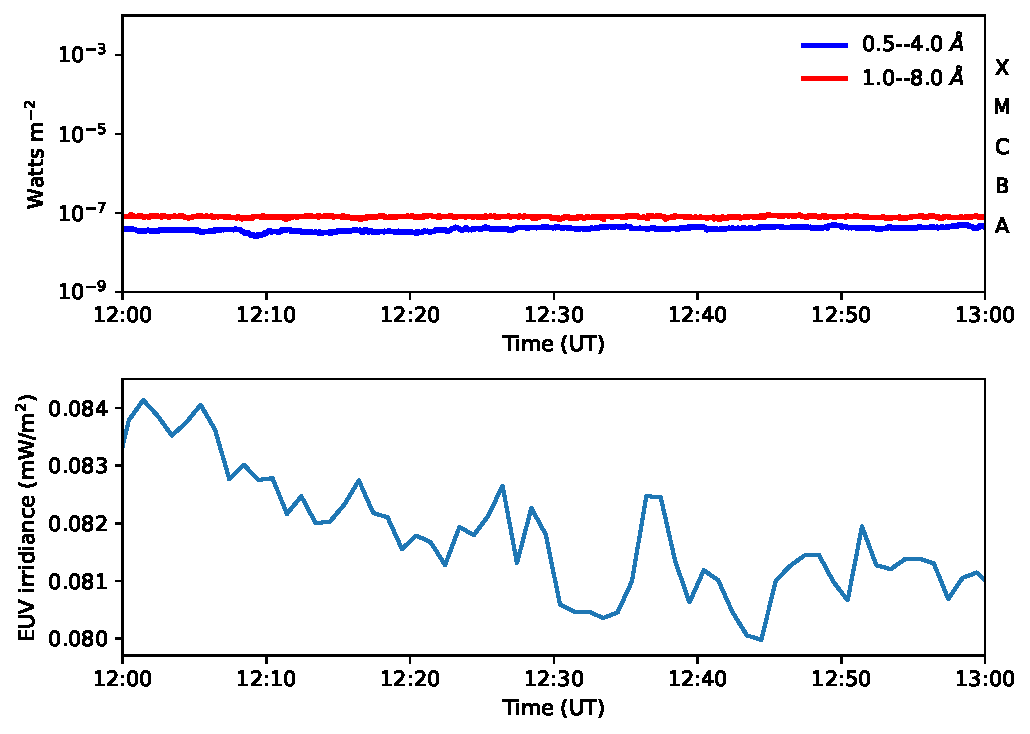
\includegraphics[width=12cm]{figs/ch2/xrs_eve.pdf}
\caption{Exploring the X-ray and extreme ultraviolet (EUV) emissions from the Sun. The top panel showcases a cutout region of the SDO/AIA 193$\AA$ image of the solar disk along with the STEREO-A EUVI 195$\AA$ point of view. The white curve is the limb of the solar disk as seen by AIA from the right side. The red and blue colors are the contours of the line-of-sight magnetogram from the SDO/HMI instrument. The levels are (50, 100, 150, 300, 500, 1000) Gauss. The middle panel shows the X-ray flux from the GOES-14 spacecraft shows minimum activity. The bottom panel shows the time series of the ESP Quad band from the SDO/EVE instrument, which shows the solar irradiance in the extreme ultraviolet (EUV) band.}
\label{soldisk_xrs}
\end{figure*}

\subsection{PSP Observations}

\subsection{LOFAR Observations}


\section{Methods}

\subsection{Imaging of radio sources}

\subsection{Modeling}


\section{Results and discussion}

\subsection{Detection and characterization of type III radio bursts}

\subsection{Imaging of radio emission sources}

\subsection{Plasma diagnostics and magnetic field analysis}


\section{Summary and conclusions}



\end{document}